\chapter{Results and Conclusions}

The injection locking was successful and we successfully produced two working beams with an adjustable detuning. 



First, we examine the output of the spectrum analyzer when we couple both Slave lasers into it. 
The two peaks clearly correspond to the two slave lasers. We can see that there is a lot of power \footnote{honestly, I'm not sure that all the power coming out was in those modes. It was a little bit flaky}
We can clearly identify which peak corresponds to which Slave laser by blocking one of the slaves. 

\section{}

Next, we attempt an experiment whereby we adjust the driving frequency. We should be able to see the peaks shifting by an amount corresponding to the change in the frequency. This will provide strong evidence that the two slaves are, in fact, injection locked to the modulated beams coming out of the AOM. 

This test has the further benefit of confirming that we have calculated the free spectral range of the cavity in the spectrum analyzer correctly. 

%where is the energy going? I think it goes from reflecting to transmitting

 
\begin{figure}
    %\centerline{\includegraphics[trim=100pt 100pt 100pt 100pt, clip=true, totalheight=0.5\textheight,angle=90]{testfigure}}
    %\centerline{\includegraphics[totalheight=0.3\textheight]{testfigure}}
    \centerline{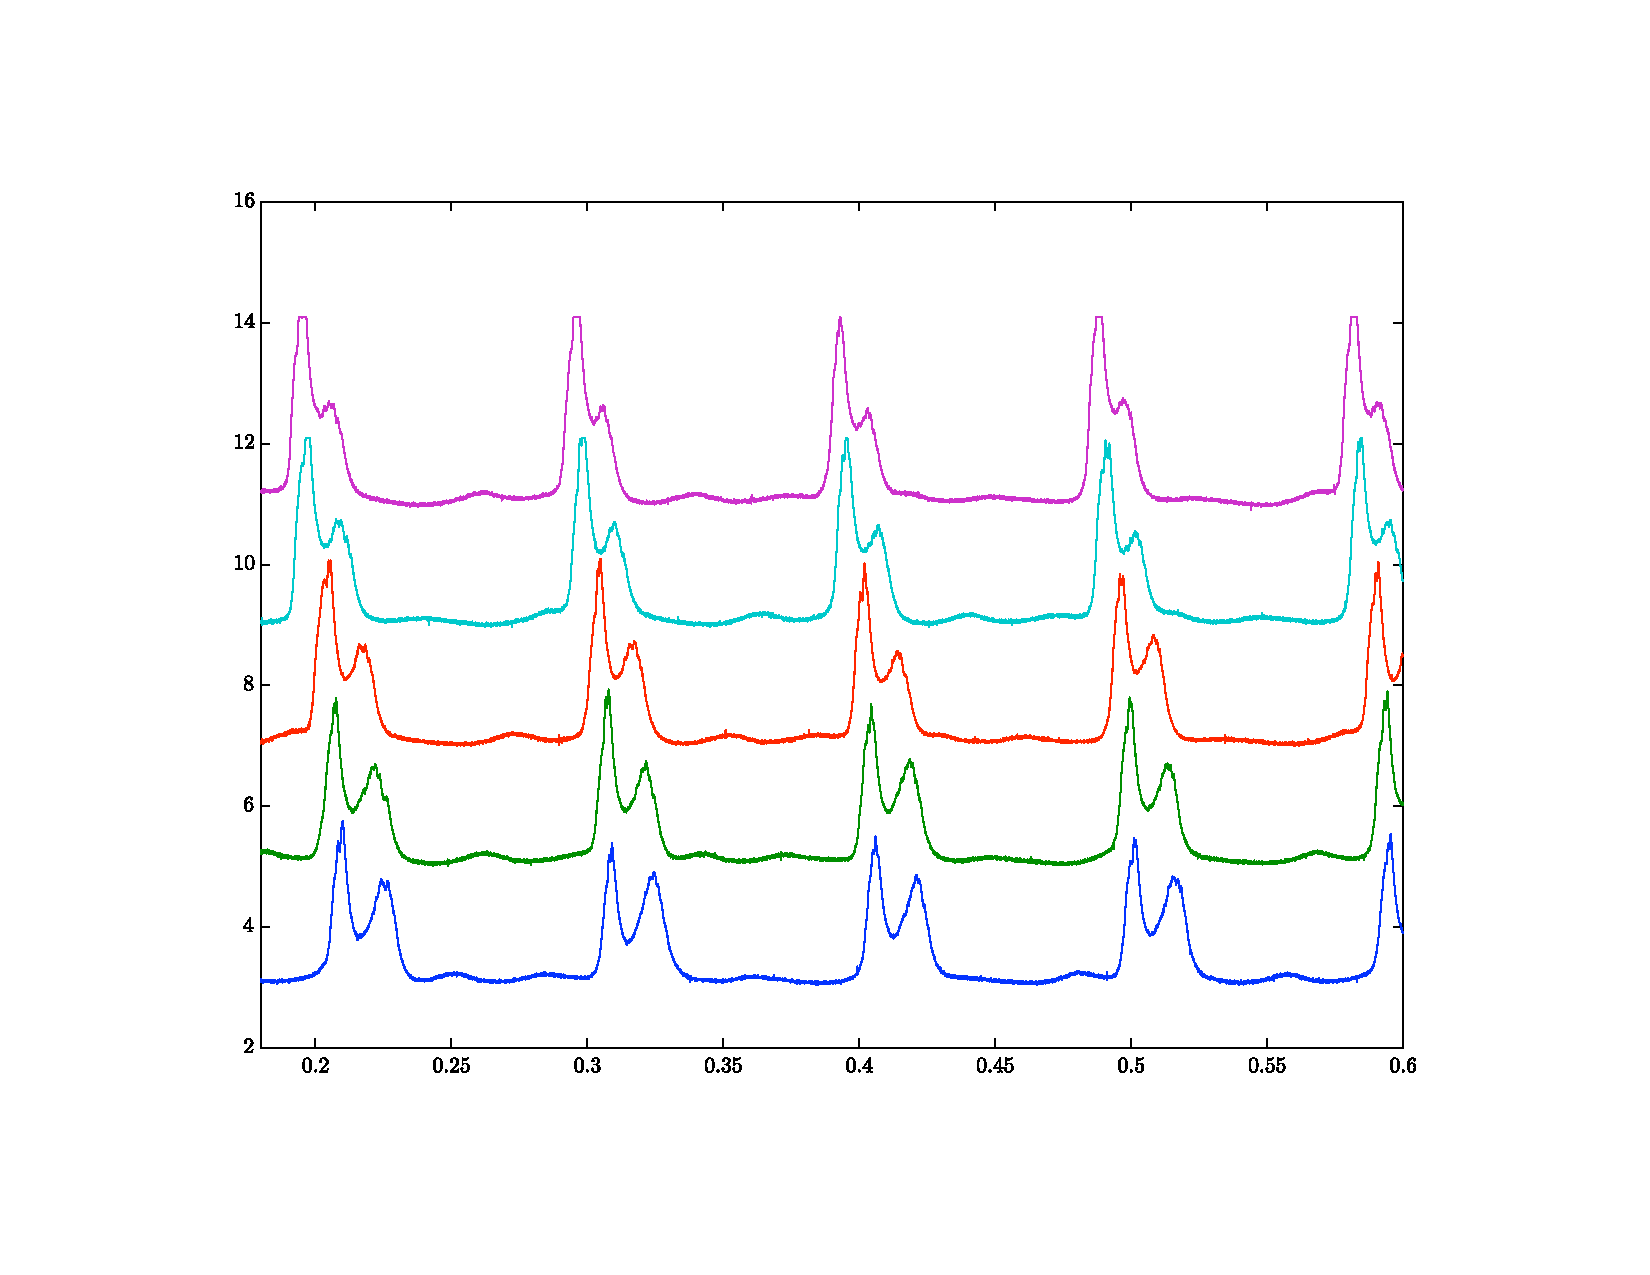
\includegraphics{sampleOffsetData}}
    %\includegraphics[totalheight=0.3\textheight]{testfigure}
    \caption[]{\label{fig:typicaldata}
    We changed the detuning on our frequency generator in something like 10 MHz increments. These are some of the data that we have that show the spacing between our peaks changing in a predictable way.}
\end{figure}
\begin{figure}
\centerline{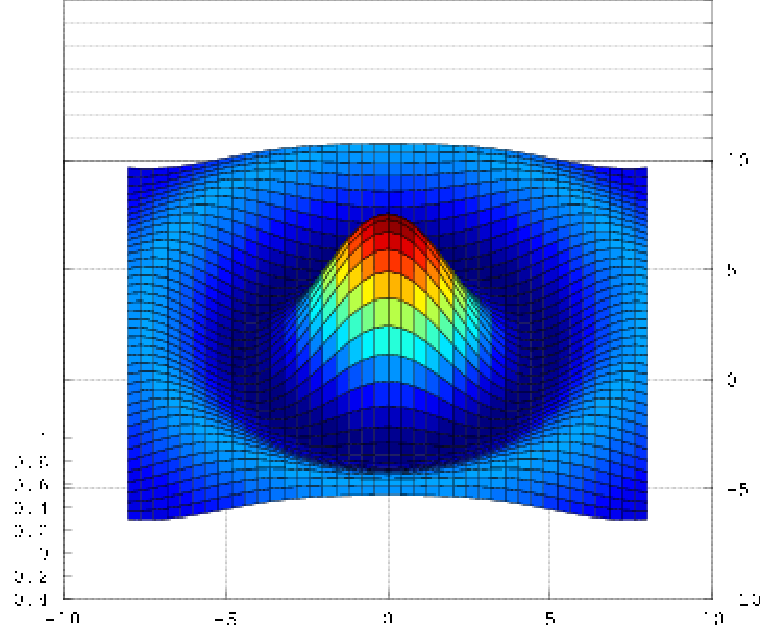
\includegraphics{thisone}}
\end{figure}

\begin{figure}
\centerline{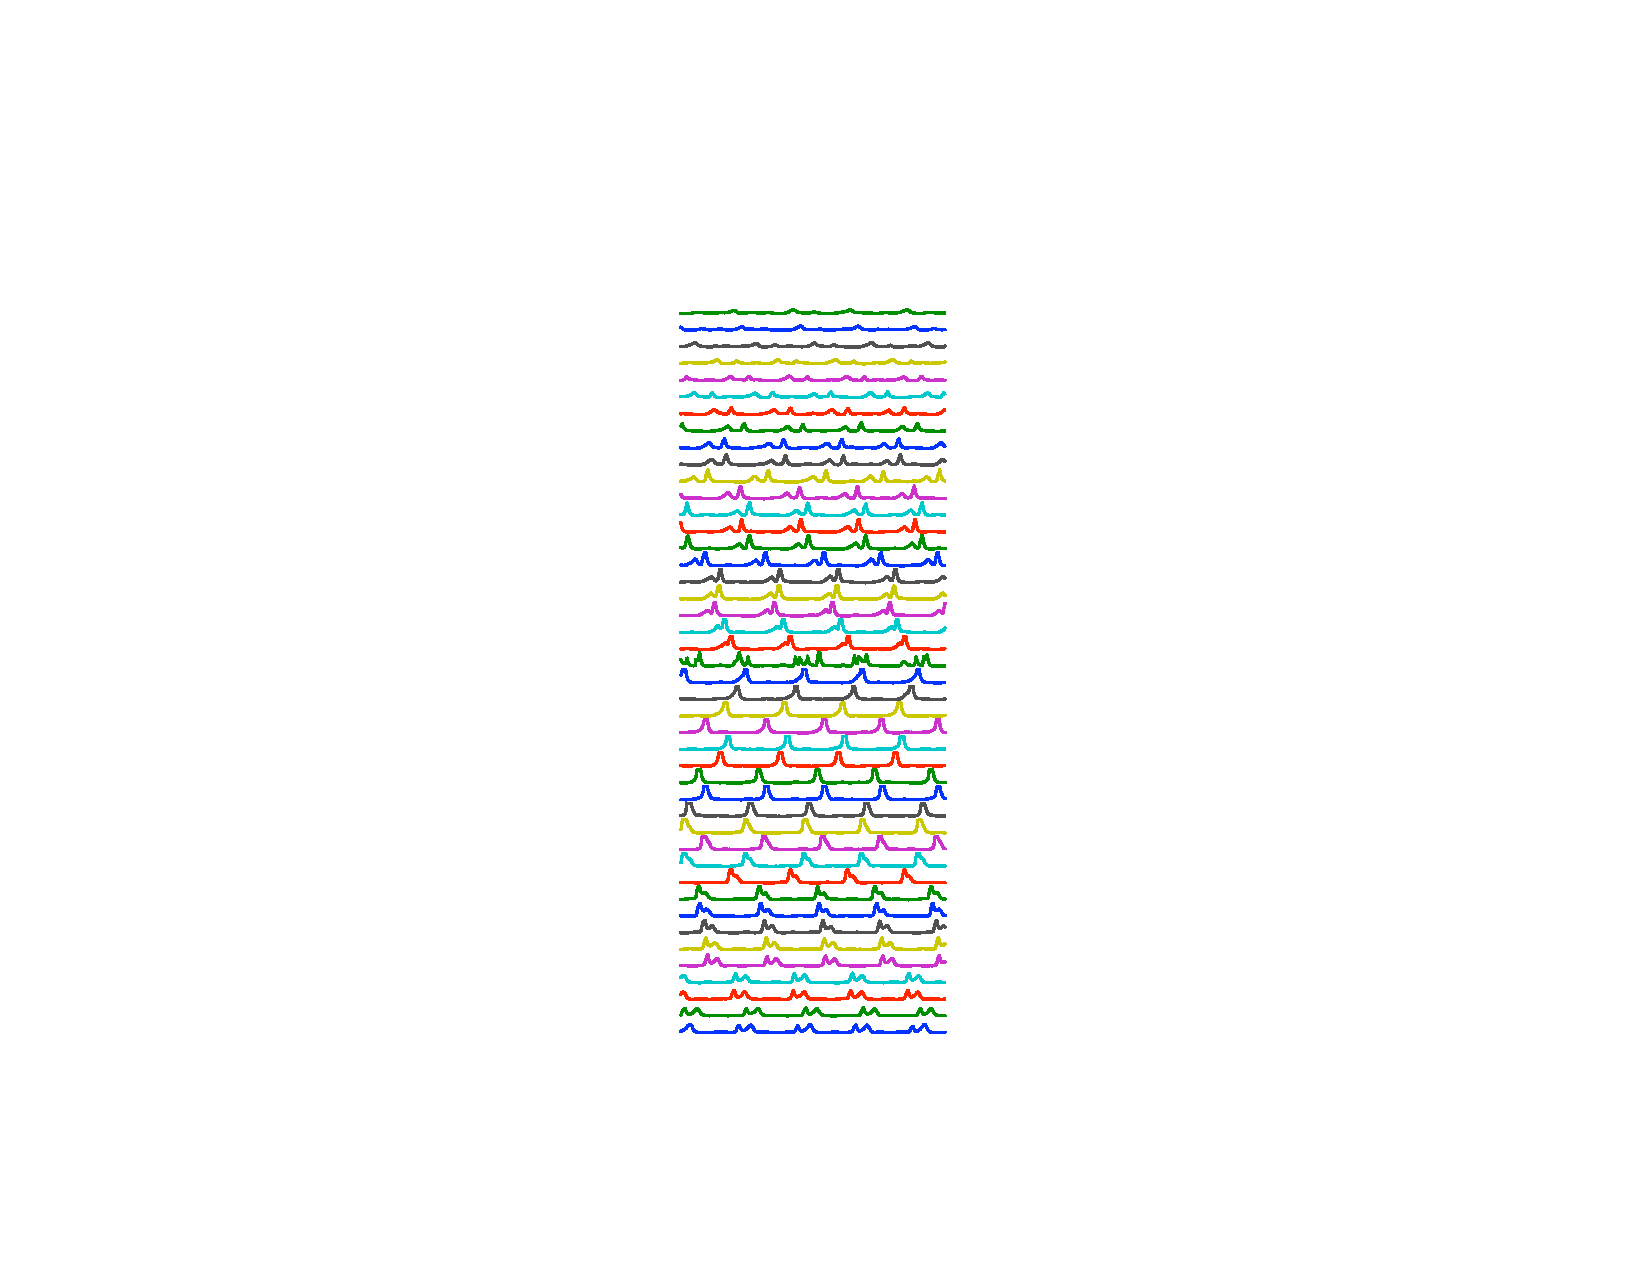
\includegraphics{all_splittingData}}
\caption[]{\label{fig:alldata} 
This is the complete set of data from which the previous graphic was culled. Some of it is clipped uglily. The peaks are on top of each other, but it may have drifted to a higher power between when I set it up and when I took the data. I'm not sure why this looks so much worse than the data I normally take.}
\end{figure}

Also, I have data that I can analyze to examine the feasibility of a Chu lock. I recorded 999 traces that showed the output of the spectrum analyzer, the current and the voltage. I recorded these over several hours, during which the laser drifted into and out of good, single mode operation. In principle, this data could be analyzed. 

We have shown that we can change the oscillator frequency and thereby change the detuning. There is a limit to the extent that we can do this. (Notice in Fig.\ \ref{fig:alldata} that the peaks get small as we continue to detune.) However, this is due to geometry. When I realigned using the method of measuring the photocurrent coming out of the slave lasers, I found that I was able to get the thing to work over an entirely different range of oscillator frequencies. 

